\chapter{Design and implementation}
\label{chap:design}

\section{System architecture}
%- Development environment (Ubuntu, WSL - Windows, RaspberryPi)
%- Hardware-software interaction (hardware setup, connections between flight controller, camera and companion computer, OS)
\todo[inline]{Interaction diagram PX4 to program}
\todo[inline]{Describe offboard API as defined by PX4}

The purpose of the Dronecontrol application is to be able to direct the movement of a \gls{uav} through the analysis of the images taken by a camera, that can be located either offboard or onboard the vehicle. 
Connected to this camera will be the companion computer that drives the image processing and control capabilities of the application.
The vehicle then interfaces directly with the companion computer using the \gls{mavlink} protocol, either through a cabled serial connection or a telemetry link between the flight controller and the companion computer.

\subsection{Offboard configuration}

In the offboard configuration the companion computer is not physically connected to flight controller but instead communicates through a telemetry radio that is connected to the flight controller's \verb|TELEM1| port and which establishes a wireless link to its matching pair connected to a USB port in the companion computer.
The radio used for the physical tests in this project is the SiK model \todo{link}, included with the Holybro X500 Kit.
More information about the exact hardware configuration used for the flight tests can be found in Chapter~\ref{chap:experimentos}.

\begin{figure}
  \centering
  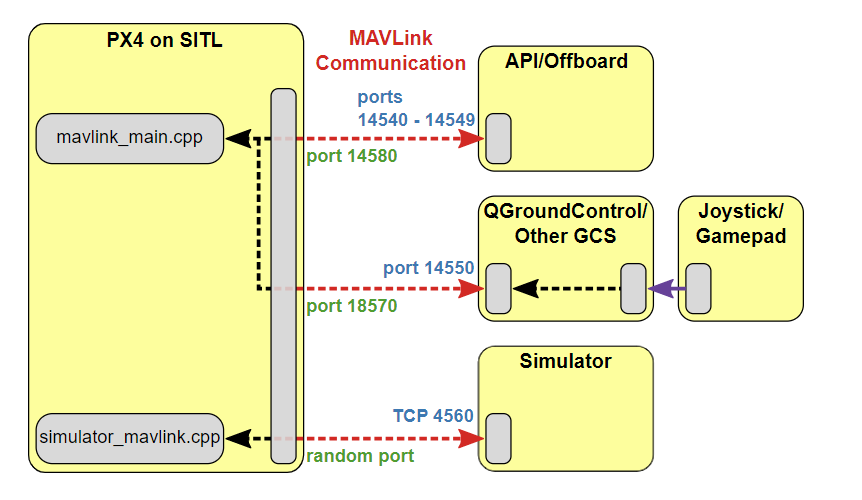
\includegraphics[keepaspectratio]{img/px4_ports.png}
  \caption{Network diagram between the different components that interconnect}\label{fig:px4_ports}
\end{figure}

Figure~\ref{fig:px4_ports} shows how the different parts of the system communicate with each other.
PX4 uses commonly established UDP ports for MAVLink communication with ground control stations (e.g. QGroundControl), Offboard APIs (e.g. MAVSDK, MAVROS) and simulator APIs (e.g. Gazebo).
External developer application like Dronecontrol use an offboard API, in this case MAVSDK, and therefore listen to PX4's remote UDP port 14540.
PX4's remote UDP Port 14550 is used for communication with ground control stations, which are expected to listen for connections on this port (QGroundControl listens to this port by default).

To connect using a telemetry radio through MAVSDK, it is only necessary to specify the radio's device address in the Linux OS, often \verb|/dev/ttyUSB0| and the port and the connection is established as if the flight controller was directly plugged to the companion computer port.
\todo{Check address and ports}
\todo{Note on latency, link frequency (915Mhz ????)}

\subsection{Onboard configuration}

The secondary way of configuring the interaction between the flight controller and the companion computer consists of integrating both together on board the \gls{uav}.
In this case, the connection is done through a direct cable between the serial port in the flight controller and a USB port in the companion computer.
The camera will then be connected via cable as well to the companion computer and oriented in the vehicle in a way that allows for the best possible perspective during flight.
This configuration makes it possible to develop new control solutions based on images taken directly from the vehicle and that reflect the trajectory that it follows.
Therefore, it becomes possible to adjust the control loop based on previous reactions of the vehicle to commands and maintain a feedback loop for a more stable guidance.

Since the computer running the visual processing algorithm now has to fly on board the vehicle, it becomes specially important to make a good choice when selecting hardware.
To be able to take into the air, the computer has to be light enough that its weight can be lifted by the propellers while maintaining an adequate battery autonomy, but also powerful enough that the processor can handle the computer vision algorithms required to extract the necessary features from the image taken from the onboard camera.

\subsection{Development environment and simulation}
During the process of developing the application, it became necessary to be able to continuously deploy and test the latest version without having to depend on flying the physical vehicle, but instead relying on the simulation of the system inside the computer that was at the same time running the developed software.
This configuration has the twofold advantage of reducing the development time on the one hand, since there is no need to be concerned with the interactions between the different hardware components and the results can be visualized immediately in the computer screen, and on the other hand of increasing the safety of the process by only running on the moving vehicle software that has already been tested to an acceptable point.

The simulation environment is composed of two differentiated parts, the first component is the simulation of the flight controller and the second is the simulation of the flight physics, with different possibilities of complexity that can be increased to include simulation of weather conditions, multi-vehicle interactions and terrain obstacles, among others.

There are many options for simulators supported by PX4 for SITL simulation.
For this project AirSim \todo{cite} was chosen for the great availability of features and ease of use, as it is based on the widely used Unreal Engine \todo{cite}, and specially for the possibility of retrieving real-time images from a simulated camera situated on the model for the vehicle to use for computer vision.
Since AirSim's native environment is Windows...

\section{Software architecture}

\begin{figure}
  \centering
  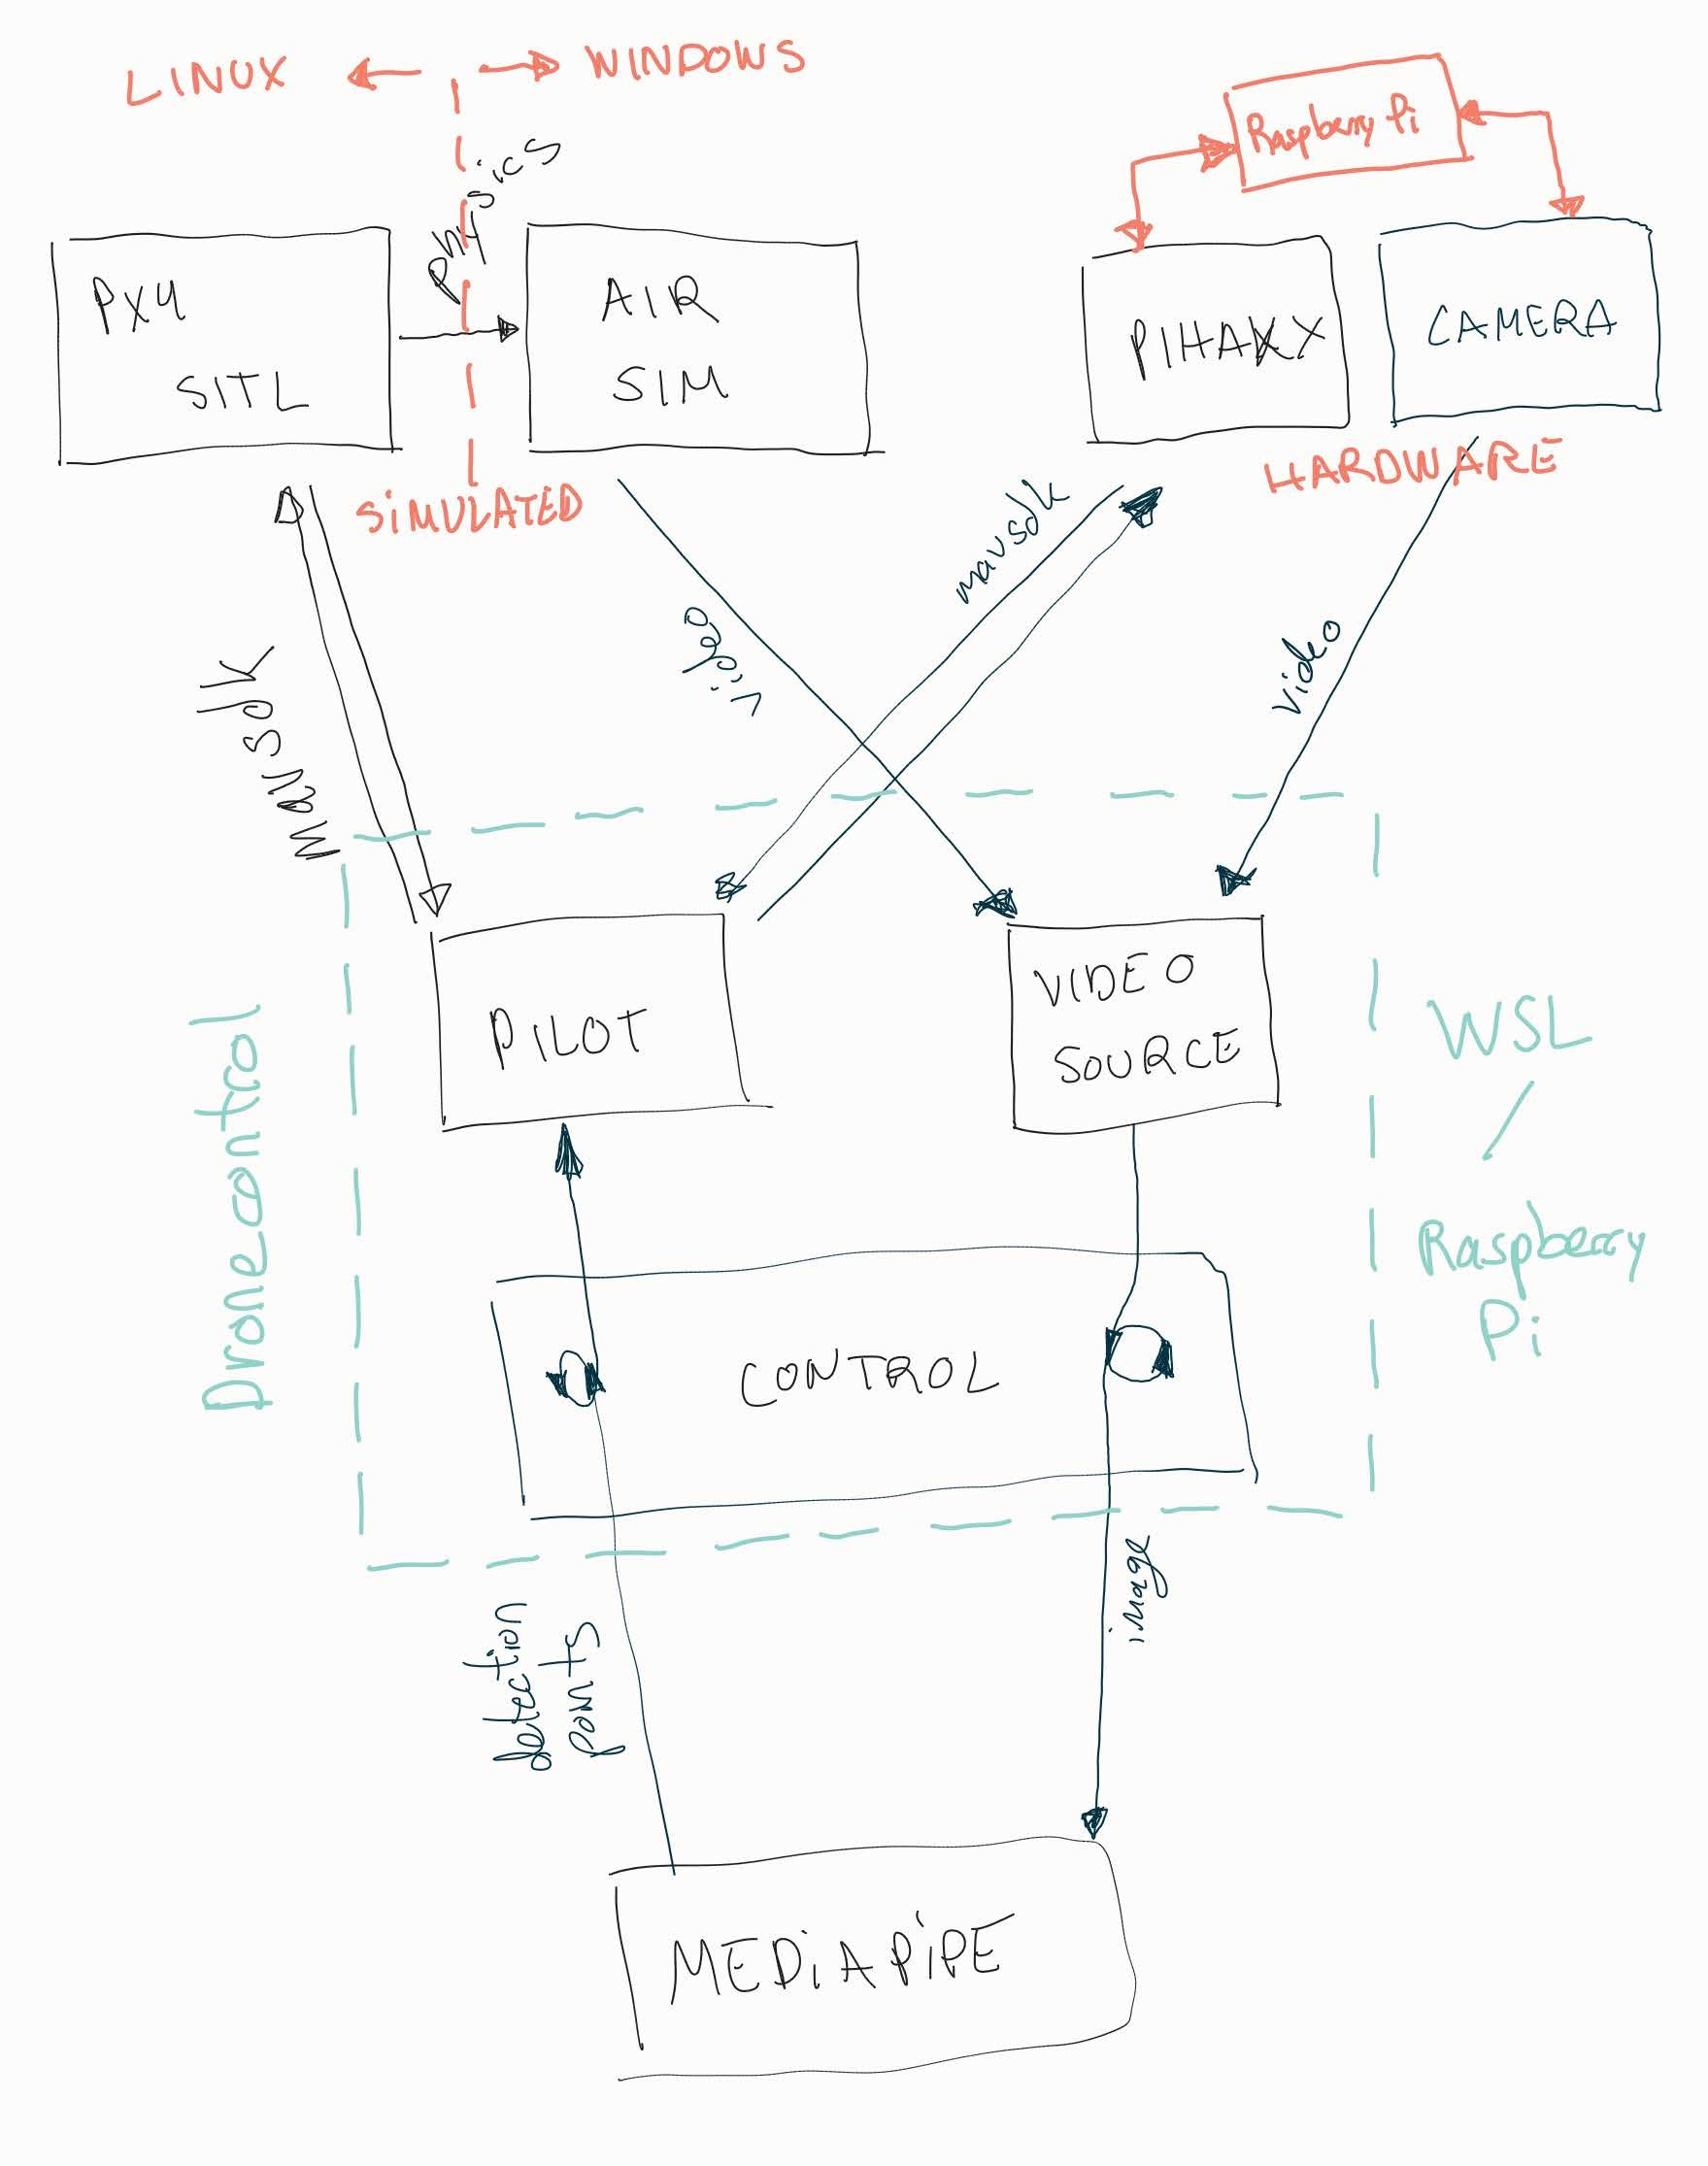
\includegraphics[width=12cm, keepaspectratio]{img/code_diagram.jpg}
  \caption{Structure of the program}\label{fig:architecture}
  \todo[inline]{Draft (use miro for final??)}
\end{figure}

Figure~\ref{fig:architecture} shows how the software is designed and how it interacts with the external libraries.
The application consists of three basic parts: 
pilot module, in charge of sending instructions to the flight controller and receiving back information on position and state through the \verb|mavsdk| library, 
a video source module that handles the retrieval of images from different sources and the necessary processing for image analysis, 
and a control module that directs the interaction between the other two to transform the pixel information first into position points through the \verb|mediapipe| library and then into instructions for the pilot.

The program can either be run in a simulated environment or control a physical unmanned aerial vehicle (UAV).
\todo{cite and explain}
In the simulation, the flight controller is simulated by PX4's software-in-the-loop system. 
In addition, a simulator with a physics engine is connected to PX4 to make it possible to see the vehicle move in real-time in the computer.
When a physical vehicle is used (for example, one with a Pihawx flight controller) the application can run either in an external companion computer that connects via a telemetry radio or in an onboard computer, like a Raspberry Pi, that connects through serial to the flight controller.
The camera required to get images to guide the vehicle is then connected directly to the computer running the application, be it on board or not.

\subsection{Pilot module}

The communication between the application and the PX4 software is done through the \verb|mavsdk| python library in the pilot module.
\emph{MAVSDK} is a collection of libraries for various programming languages to interface with MAVLink systems such as drones, cameras or ground systems.
The libraries provides a simple API for managing one or more vehicles, providing programmatic access to vehicle information and telemetry, and control over missions, movement and other operations.
The libraries can be used onboard a drone on a companion computer or on the ground for a ground station or mobile device.
\emph{MAVSDK} is primarly written in C++ with wrappers available for several programming languages.
The Python wrapper is based on a gRPC (Google Remote Procedure Call) client communicating with the gRPC server written in C++.
MavSDK provides an asynchronous API to be able to run coroutines in parallel while waiting for the messages provided through the \emph{MAVLink} communication.

Therefore it requires the use of library to write concurrent code, like the Python standard library \verb|asyncio|, 
that provides support for it using the \verb|async/await| syntax.
\verb|asyncio| is used as a foundation for multiple Python asynchronous frameworks that provide high-performance network and web-servers, database connection libraries, distributed task queues, etc; 
and provides a set of high-level APIs to run Python coroutines concurrently and have full control over their execution.
The pilot module integrates \verb|mavsdk| and \verb|asyncio| and provides a queue for the control module to send actions to be executed in the vehicle one after another.

\subsection{Video source module}

The objective of the video source module is to provide a collection of classes to retrieve images from different sources,
in a way that they can be exchanged for one another without affecting the rest of the application to facilitate testing and be adaptable running in different environments.
There are three classes of video sources implemented: file, simulator and camera.

The file source provides images processed from a video file stored in the companion computer.
The simulator source uses AirSim's Python library to communicate with the simulator and retrieve images from a simulated camera attached to the 3D model of the vehicle in Unreal Engine.
The camera source uses OpenCV, which provides drivers to access the images recorded by a physical camera attached to the computer running the application, for example via USB.

\subsection{Control module}
Something, something, something, ... The next two sections offer a more complete explanation of the control module used by the two different solutions developed.

% Config, venv, programs

\section{First steps: hand-gesture solution}

\section{Final solution: human following}

%\section{Hardware-software interaction}


\cleardoublepage